\chapter{Auswertung}
\section{Messung des Übertragungsverhaltens}
	\begin{gnuplot}[terminal=pdf,terminaloptions={font ",10" linewidth 3},scale=1.2]
	
	set xlabel "Frequenz f [kHz]"
	set ylabel "Normierte Ausgangsspannung U [V]"
    f(x)=a*exp(-b*x)
   	set logscale y
    set logscale x
    
    fit f(x) 'Daten/1.csv' using ($1/1000):($3/1000)/$2 via a,b
	plot 'Daten/1.csv' using ($1/1000):($3/1000)/$2 t "Spannung", f(x) t "U(f)"
    
	\end{gnuplot}
    \label{Messwert1}
    \captionof{figure}[Messwert1]{Das Verhalten des Komplexen Spannungsteilers}
    \ \\
	Die gemessene Ausgangsspannung wird mit den gemessenen Eingangsspannungen normiert. In Abbildung \ref{Messwert1} ist der Quotient $\frac{U_a}{U_e}$ über die Frequenz $f$ in einem Bode-Diagramm aufgetragen.\\ 
    An die Messdaten wird eine Fitfunktion der Form 
    \begin{equation}
    	U(f)= a\cdot\exp(b\cdot f)
    \end{equation}
    angefittet. Der Koeffizient $a$ entspricht dabei $\frac{U_a}{U_e}$. Über Gnuplot werden die Koeffizienten $a$ und $b$ bestimmt.
    \begin{center}
    	\begin{tabular}{c|c}
    	Koeffizient & Wert \\\hline
        $a$ & $0,7365$\\
        $b$ & $0,2107$
    	\end{tabular}
    \end{center}
	Für $f \rightarrow 0$ verschwindet der komplexe Widerstand der Spule und es kann der ohmsche Widerstand über den Spannungsteiler bestimmt werden. 	\\
    Im Stromkreis gilt 
\begin{align*}
	R_{sp} &= R_{ges}-R \\
    & =  \frac{U_e}{I} - R \\
    & = \frac{U_e}{U_a / R} - R \\
    & =  R\cdot \left(\frac{U_e}{U_a} -1\right)
\end{align*}
    und für den Widerstandswert 
    \begin{align*}
	R_{sp} &= R\cdot \left(\frac{U_e}{U_a} -1\right) \\
   	& =  (1 \Omega) \cdot (\frac{1}{0,7365} - 1) =  0,3578 \Omega
\end{align*}
    Alternativ kann der ohmsche Widerstand auch über den spezifischen Widerstand berechnet werden mit Formel \eqref{spezifischerWiderstand} \\
    Mit $l = \pi \cdot d \cdot n_a$ und $A = \pi \cdot \frac{1}{4} d^2$ ist
    \begin{align*}
    	R_{sp}&=\rho\cdot\frac{\pi\cdot 2 r\cdot n_a}{\pi\cdot\frac{1}{4}\cdot d^2} = \rho\cdot\frac{8\cdot r\cdot n_a}{d^2} \\
        &=0,017 \frac{\Omega mm^2}{m}\cdot\frac{8\cdot 0,025m \cdot 117}{(1mm)^2} =  0,3978 \Omega
	\end{align*}
    
    Außerdem kann der komplexe Spannungsteiler betrachtet werden. Es gilt das Verhältnis \begin{align}
    \frac{U_a}{U_e} = \frac{R}{R_{ges}} = \frac{R}{|Z_{ges}|} = \frac{R}{\sqrt{(R + R_{sp})^2 + (\omega L)^2}}
    \end{align}
    Die Formel (5.2) zeigt, was in Abbildung 5.1 vor sich geht. Für kleine $\omega$ kann der Term $(\omega L)^2$ vernachlässigt werden und man erhält das normale Ohmsche Gesetz. Für sehr große $\omega$ wird jedoch der Term $R + R_{sp}$ vernachlässigbar und der Blindwiderstand dominiert den Spannungsteiler. Die Vereinfachung für kleine Frequenzen wird bereits bei der Berechnung des ohmschen Widerstandes der Spule weiter oben ausgenutzt. Nun wird für große Frequenzen die Induktivität bestimmt. Für die höchste gemessene Frequenz gilt:
    \begin{align*}
    	\frac{U_a}{U_e} &= \frac{R}{(\omega L)^2} \\
    	L & = \sqrt{\frac{U_e \cdot R}{U_a \cdot \omega^2}} \\
    &= \sqrt{48,18 \cdot\frac{1 \Omega}{60\cdot 10^3 Hz}} = 0,8 \cdot 10^{-3} H 
    \end{align*} 
    \section{Verlauf des magnetischen Feldes}
   Mit Formel (3.1) berechnet man das B-Feld. Tabelle 5.1 enthält die Ergebnisse und Abbildung 5.2 zeigt das B-Feld über die Entfernung zum Mittelpunkt der Spule aufgetragen.
     \begin{equation}
		B_{0cm} =\frac{1}{2 \pi 100Hz \cdot 1000 \cdot 0,00035m^2} \cdot 0,13 V = 591,15 \cdot 10^{-6} H
	\end{equation}
    Analog für die restlichen Werte.
    \begin{center}
\captionof{table}[]{Induzierte Spannung im inneren der Spule}
\begin{tabular}{c|c||c|c}
$z[cm]$ & $B [\mu H]$ &$z[cm]$ & $B [\mu H]$ \\ \hline\hline
0& 591,15 & 14& 85,49 \\
1& 604,79 & 15& 55,02 \\
2& 600,24 & 16& 36,74 \\
3& 591,15 & 17& 26,15 \\
4& 586,60 & 18& 19,78 \\
5& 591,15 & 19& 15,10 \\
6& 582,05 & 20& 11,87 \\
7& 577,51 & 21& 9,55  \\
8& 559,32 & 22& 7,96 \\
9& 532,03 & 23& 6,59 \\
10& 477,46 & 24& 5,64 \\
11& 378,33 & 25& 4,77 \\
12& 242,82 & 26& 0.04 \\
13& 148,24 &  &
\end{tabular}\end{center}
\begin{gnuplot}[terminal=pdf,terminaloptions={font ",10" linewidth 3},scale=1.2]
	
	set xlabel "Abstand z [cm]"
	set ylabel "Magnetisches Feld B [Wb]"
    f(x) = a*x +c
    fit f(x) "Daten/2.csv" u 1:4 via a,c
	set arrow from 11.65,0 to 11.65,0.0007
	plot 'Daten/2.csv' using 1:3 t "Magnetfeldstärke"
    
	\end{gnuplot}
    \captionof{figure}[DurchlassGerSil]{Stärke des Magnetfeldes der Spule}
\ \\
Es wird keine Messung am Ende der Spule durchgeführt, man kann jedoch den Wert extrapolieren. Legt man mit Gnuplot eine Gerade an den Teil des Graphen, in dem sich die gesuchte Stelle befindet, so ergibt sich ein Wert von etwa $0,29 \cdot 10^{-3} Wb$
\section{Frequenzabhängigkeit der Induktionsspannung}
\begin{gnuplot}[terminal=pdf,terminaloptions={font ",10" linewidth 3},scale=1.2]
	
	set xlabel "Frequenz f [Hz]"
	set ylabel "Normierte Ausgangsspannung U [V]"
    f(x)=a*x+b
    
    
    fit f(x) 'Daten/3.csv' using 1:2 via a,b
    
	plot 'Daten/3.csv' using 1:2 t "Spannung", f(x)  "U(f)"
    
	\end{gnuplot}
    \captionof{figure}[DurchlassGerSil]{Messungen der Abhängigkeit von Frequenz und Spannung} \ \\
    Man erkennt deutlich den linearen Zusammenhang zwischen der Frequenz $f$ der Wechselspannung und der induzierten Spannung $U_{ind}$. Ein Blick auf die Theorie bestätigt diese Beobachtung durch Formel (3.1).
   
\section{Untersuchung der Form der Induktionsspannung}
Es wird erwartet, dass die induzierte Spannung sich wie die Ableitung der Quellspannung (skaliert um den effektiven Strom) verhält.
Abbildung 5.4 zeigt eine Sinus-Eingangs-Spannung, bei der die induzierte Spannung einem Cosinus entspricht. Das kann man sich leicht klarmachen, da am Umkehrpunkt der Eingangsspannung die größte Änderung auftritt und so den höchten Strom induziert.
In Abbildung 5.5 wird eine Dreiecksspannung verwendet. Ihre Flanken mit konstanter Steigung treten in der induzierten Spannung als Konstanten auf, die eine Rechteckspannung beschreiben.

Abbildung 5.6 zeigt die Induktion einer Rechteckspannung. Mathematisch gesehen haben die Flanken der Rechteckspannung eine unendliche Steigung. Dies lässt sich mathematisch mit einer Kombination von Delta-Distributionen darstellen. In der Induktionsspannung stellt es sich als sehr enge "Peaks" dar, da physikalisch keine Änderung in einer unendlich kurzen Zeit passieren kann \\
\begin{multicols}{3}[Vergleich der Signalformen][3px]
\begin{center}
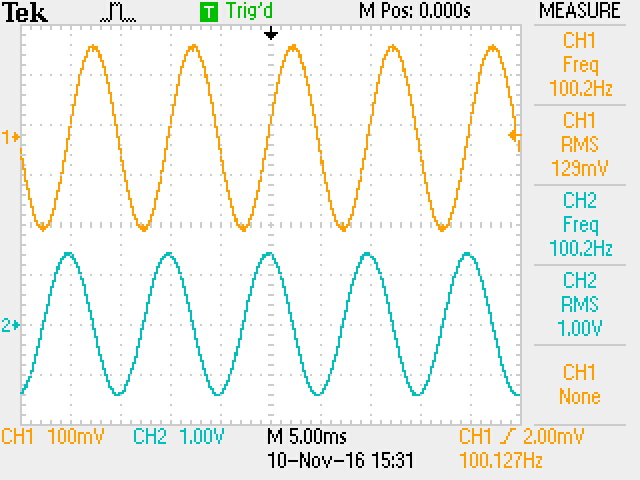
\includegraphics[scale=0.5]{Daten/sinus.JPG}
  \captionof{figure}[]{Entstörte Sinus-Spannung}
  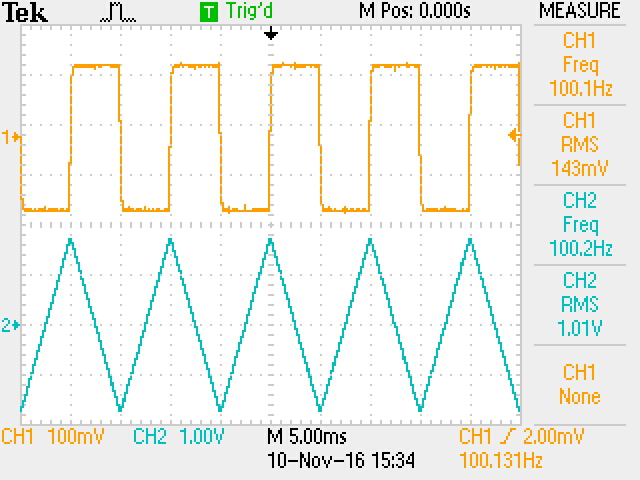
\includegraphics[scale=0.5]{Daten/Dreieck.JPG}
  \captionof{figure}[]{Dreick-Spannung}
  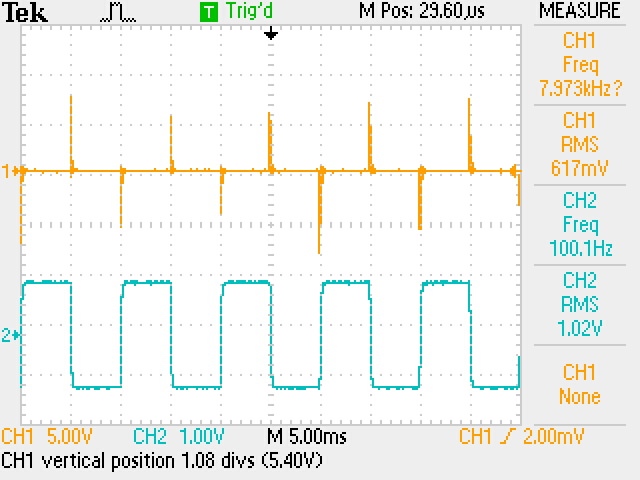
\includegraphics[scale=0.5]{Daten/Rechteck.JPG}
  \captionof{figure}[]{Rechteck-Spannung}
\end{center}
\end{multicols}

Bei genauerer Untersuchung des Rechtecksignales fällt auf, dass nach einer Spannungsspitze ein oszillierendes Signal bleibt, welches sich nicht durch die Induktivität der Spule allein erklären lässt. Die wahrscheinlichste Erklärung ist, dass die Induktivität der Spule zusammen mit der Kapazität des Oszilloskopeingangs einen Schwingkreis bildet. So kann die Induktivität der Spule bestimmmt werden. Aus Abbildung 5.7 ergibt die Frequenz $f=87,87 kHz$ ablesen.\\
Mit der Formel
\begin{equation}
	f  = \frac{1}{2\pi\cdot\sqrt{ L\cdot C}}
\end{equation}
gilt für die Induktivität L
\begin{align*}
	  L &= \frac{1}{f^2 \cdot 4\pi^2 \cdot C} \\
      &= \frac{1}{(87,87 \cdot 10^{3} Hz)^2 \cdot 4\pi^2 \cdot (110 \cdot 10^{-9} F)} \\
      &  \approx 3 \cdot 10^{-5} H
\end{align*}

\begin{center}
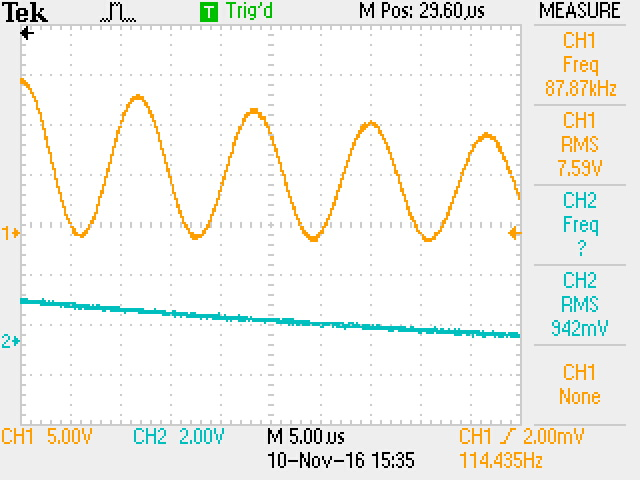
\includegraphics[scale=0.8]{Daten/Oszillation.JPG}
  \captionof{figure}[]{Oszillationen an der Rechteckspannung} 
\end{center}
  
\section{Untersuchung der Selbstinduktion}
  Weiterhin wird untersucht, wie sich die Spannung kurz nach dem Einschaltvorgang (Ausschaltvorgang) verhält. Zur Simulation dieser Vorgänge wird eine Rechteckspannung eingespeist. In Abbildung 5.8 ist zu erkennen, das die Spannung nach dem Umschalten mit einer Verzögerung ansteigt. Mit einer kurzgeschlossenen Spule Abbildung 5.9 sind keine Anstiegskurven mehr zu erkennen. Die Theorie erklärt, dass das in der Spule entstehende Magnetfeld einen umgekehrt gepolten Induktionsstrom in sich selbst erzeugt und so dem erzeugenden Strom entgegenwirkt. Wird die Spule kurzgeschlossen, kann der Strom ungehindert fließen.
\begin{multicols}{2}[Vergleich der Ein- und Ausschaltvorgänge][3px]
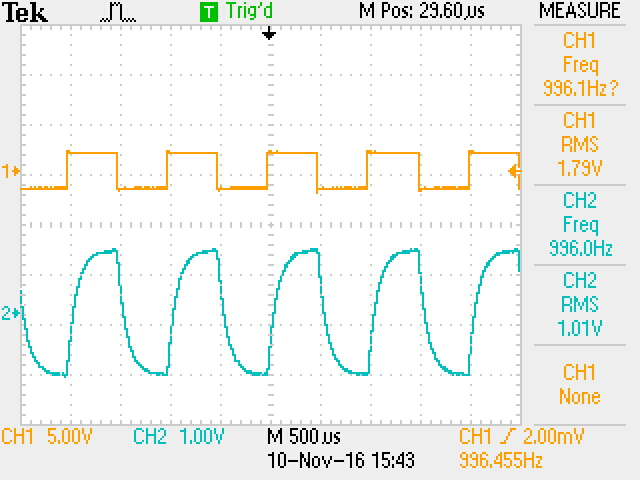
\includegraphics[scale=0.8]{Daten/ohneKurzschluss.JPG}
  \captionof{figure}[]{Kein Kurzschluss} 
  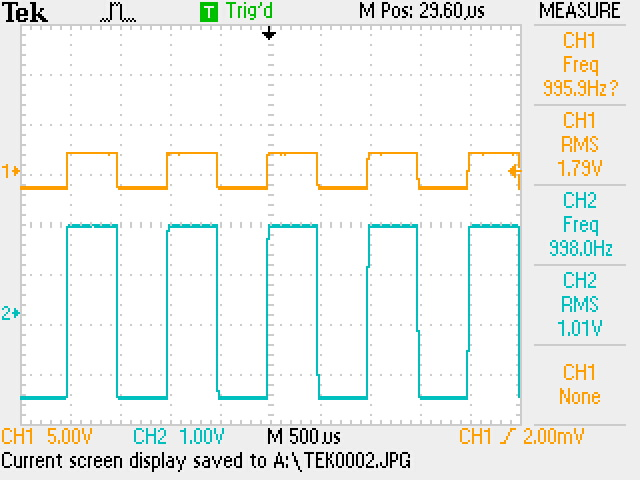
\includegraphics[scale=0.8]{Daten/mitKurzschluss.JPG}
  \captionof{figure}[]{Kurzschluss}
\end{multicols}
  
    \pagebreak